\chapter{Symbol Tables}

Here we will improve our symbol table notion to make it more robust,
especially to prepare for functions.

\section{Rationale}

When we introduced variables, we started using the simplest possible
symbol table: a dictionary mapping name to value. As the complexity
of the language increases, we will need more and more from our symbol
table.

For instance, when we introduce functions, users will be very surprised
if the variables defined as function parameters are in the symbol
table for use before or after the function is called. Almost all languages
have a notion of scope. The scope is the set of statements from which
a particular variable is accessible (another word for accessible is visible).

Global variables are a bane. Their presence invites unexpected collisions
that result in surprising values. Limiting scope is a key feature of
languages. Yet, for a simple language like ours, some globals make sense.
Much of our code is not in a block. The variables we use outside of all
blocks are going to be global.

At the other extreme, Java has no global scope at all. Every variable
must belong to a class, enum, or interface. All code must be in a
method. It also restricts variables declared within a block to that
block. Python doesn't have these limitations, but it still has
scoping. In it, a variable comes into existence with its first assignment
and is visible within the rest of the function. There are lots of other
variations. But, the modern concensus is that scoping is helpful to
retain sanity and prevent errors at a distance.

\section{Block Scoping}

Not all languages introduce a scope with each block, but it is a feature
I prefer. My favorite language is Perl. In it you can use a bare
block just to create a limited scope.

Even when we introduce block scoping, we still want to see variables
from the outer scopes. This requires making at least a stack of symbol
tables. I chose a linked list to implement that stack for our language.
Then, simple reference management creates and restores inherited scopes
at block entry and exit. This structure is also easy to extend. To
work for function scopes it will become a tree.

To achieve the stack, I created a new class called SymbolTable. It has
a dictionary in it, but also a reference to a previous scope. When we
are about to enter a block, we create a new table that refers to the
current scope as its previous scope. When the scope ends, we use the previous
reference to restore the original table. When looking up a variable, we
check the current scope first. But, if we can't find it there, we scan
the ancestors. Only if none of the scopes have it do we complain.

When we assign values to variables, we will also scan the scopes looking
for an existing version of the variable. If we find one, we update it.
Otherwise, we make a new one in the current scope.

There are other choices. We could introduce a declaration statement,
separate from assignment. Then all declarations would go into the
current scope. Lookups and assignments would still scan up the scope
stack. These are language design decisions. Feel free to make different
ones than I made.

This is my first attempt at a symbol table class.

% SymbolTable.py (stages/04fuctions) but without the caller pointer

{\footnotesize
\begin{verbatim}
    class SymbolTable:
        def __init__(self, previous):
            self.symbols = {}
            self.previous = previous
\end{verbatim}
}

Here we see the current table as the symbols dictionary attribute.
Its immediate outer scope (if there is one) is the previous reference,
which points to the other SymbolTable object.

{\footnotesize
\begin{verbatim}
        def addInnerScope(self):
            return SymbolTable(self)

        def discardInnerScope(self):
            return self.previous
\end{verbatim}
}

When we are about to enter a block, we will replace our current table
with the one returned by addInnerScope. Note that it passes its own
reference (self) to the constructor to become previous for the new table.

When the block is finished, we call discardInnerScope and replace the
current table with the previous one that it returns.

The caller must replace its current symbol table with the return values
of these functions.

To store values in the symbol table in the visitor, we stop directly
accessing the dictionary and start calling methods on the SymbolTable.
These methods are set (to assign or update) and resolve (to lookup).

{\footnotesize
\begin{verbatim}
        def set(self, name, value):
            homeTable = self._findTable(name)
            if homeTable == None:
                self.symbols[name] = value
            else:
                homeTable.symbols[name] = value
\end{verbatim}
}

To set a variable, we need the name and the new value. The
\verb+_findTable+ method
returns the table where the variable already exists or
None.\footnote{Python uses None for its null, aka undefined, value.}
If we haven't seen the variable before, it goes into the
table in the current object instance. Else, its value in its home table
is updated.

{\footnotesize
\begin{verbatim}
        def resolve(self, name):
            homeTable = self._findTable(name)
            if homeTable == None:
                raise Exception("No such symbol " + name)
            else:
                return homeTable.symbols[name]
\end{verbatim}
}

Similarly, resolve uses \verb+_findTable+ to locate the variable. But, if
it is not found, we need to complain. This is a fatal exception.

The \verb+_findTable+ method walks the list of tables looking for the variable.

{\footnotesize
\begin{verbatim}
        def _findTable(self, name):
            try:
                value = self.symbols[name]
                return self
            except:
                if self.previous != None:
                    return self.previous._findTable(name)
                else:
                    return None
\end{verbatim}
}

This takes advantage of python's exception mechanism for dictionary lookups.
Asking for a key that is not in the dictionary raises an exception.
This is jarring for some of us who expect exceptions to mean something
is catastrophically wrong. Python sometimes uses exceptions as a flow
of control mechanism.

If the lookup works, we return the current table. Otherwise, we
check to see if there is a previous table. If there is one, se
call \verb+_findTable+ on it. When we reach the original global table, the
one with no previous table, we return None. Remember that set and
resolve respond to this differently. For set, it means we are declaring
the variable in the current scope. For resolve, it means we have
not seen the variable, which is a fatal error.

So far, we have a structure like this, when we are in a nested block.

\begin{figure}
\centering
%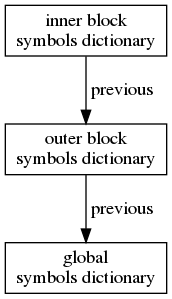
\includegraphics[scale=.35]{blockscopesymboltable.png}
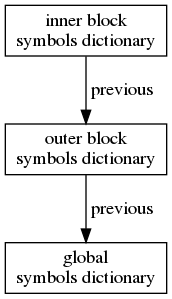
\includegraphics{blockscopesymboltable.png}
\end{figure}

\section{Function Scoping}

The approach in the previous section wears out when we arrive at
functions. A function block should still be able to see global variables.
But, if we call it from within a block, it should not
see the variables in scope for the caller. This is doubly true if the
function calls a function. They should have separate scopes, both
of which can see the global symbols, but not the one belonging to
the other function invocations. To understand the problem, think of
a recursive function. Each invocation needs separate symbols, which
will necessarily have the same names.

To fix this, we need minor changes to the SymbolTable class. First,
we need to add a reference to the caller, which will store the
table in scope at the point of function invocation. Then, we
need new methods to add and discard function scopes.

The only changes to existing code are these

{\footnotesize
\begin{verbatim}
    class SymbolTable:
        def __init__(self, previous, caller):
            self.symbols = {}
            self.previous = previous
            self.caller = caller

        def addInnerScope(self):
            return SymbolTable(self, None)
\end{verbatim}
}

The constructor receives and stores the caller reference. In
addInnerScope we need to pass that parameter, but None works for
regular scopes which have no caller.

There are two new methods for function scope management.

{\footnotesize
\begin{verbatim}
        def addFunctionScope(self, globalTable):
            return SymbolTable(globalTable, self)

        def discardFunctionScope(self):
            return self.caller
\end{verbatim}
}

We make a new scope by constructing with the global table
as previous and the current scope as the caller. Discarding just
returns the caller reference to put the original scope back. Nothing
else changes.

Note that the visitor will need to call these methods correctly and
store their return values.

To see what the symbol table structure looks like with these changes,
consider this example program:

{\footnotesize
\begin{verbatim}
    fun callAdd(a) {
        if (a > 2) {
            return 3 * a
        }
    }

    if (x > 4) {
        while (x > 4) {
            total = callAdd(x)
            x = x - 1
        }
    }
\end{verbatim}
}

Then the full set of symbol tables inside the if in callAdd looks like
this:

\begin{figure}
\centering
%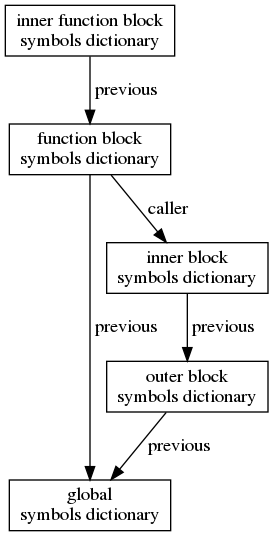
\includegraphics[scale=.35]{functionscopesymboltable.png}
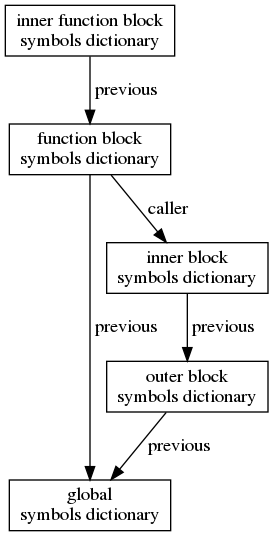
\includegraphics{functionscopesymboltable.png}
\end{figure}

\section{Exercises}

\subsection{Visitor Implemenation}

Create the SymbolTable class and use it to create block scopes
in your existing visitIf and visitWhile methods (in Visitor). You
may need to adjust tests to define variables before scopes begin.

\subsection{Debugging}

Add a debugging method to the SymbolTable class which draws the
structure.
Call the method at strategic points to see the structure grow and
shrink as scopes are added and removed.
Hint: we really have is almost a binary tree now with previous
as the left pointer and caller as the right pointer. There are not
cycles in this graph, but many roads lead to the global table.

\subsection{Testing}

Add a TestSymbolTable class to test the behaviors of the SymbolTable class.
